\documentclass{beamer}
\usepackage[T1]{fontenc}
\usepackage[utf8]{inputenc}
\usepackage[francais]{babel}
\usepackage{lmodern}
%\usepackage{url}
\usepackage{graphicx}
\usepackage{amssymb}

\title{La disposition de clavier Dvorak bépo}
\author{Sébastien Wilmet}
\date{8 mars 2011}
\institute{LouviLUG}

\usetheme{Warsaw}

\begin{document}

\begin{frame}
  \titlepage
\end{frame}

\begin{frame}{Sommaire}
  \tableofcontents[hideallsubsections]
\end{frame}

%%%%%%%%%%%%%%%%%%%%%%%%%%%%%%%%%%%%%%%%%%%%%%%%%%%%%%%%%%%%%%%%%%%%%%%%%%%%%%%
\section{Les machines à écrire}
\begin{frame}
  \tableofcontents[sectionstyle=show/shaded, hideothersubsections]
\end{frame}

\subsection{Purement mécanique}
\begin{frame}{Purement mécanique}
\begin{center}
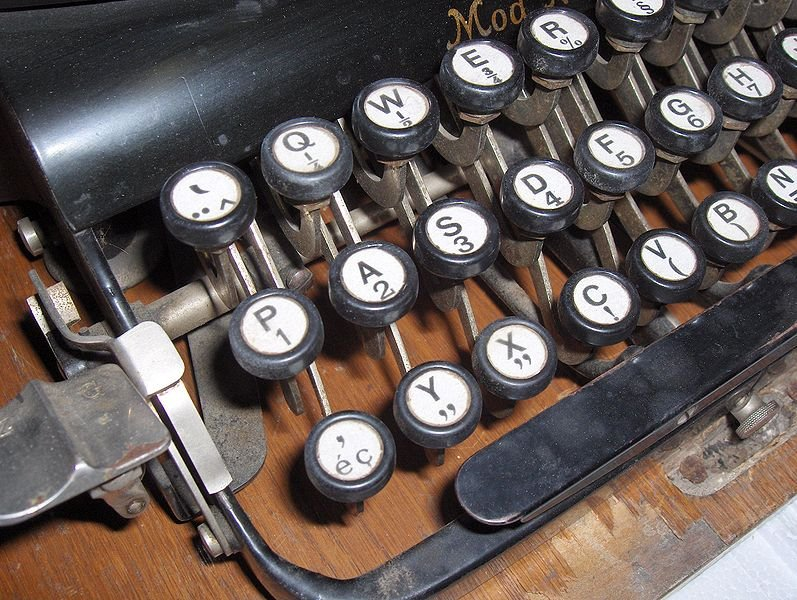
\includegraphics[height=6cm]{machine-a-ecrire.jpg}
\end{center}
\end{frame}

\subsection{Petit problème…}
\begin{frame}{Petit problème…}
\begin{center}
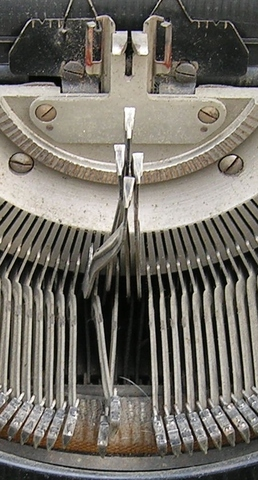
\includegraphics[height=6cm]{barres-coincees.jpg}
\end{center}
\end{frame}

\subsection{Solutions}
\begin{frame}{Solution : touches en diagonale}
Inconvénient : on fait plein de fautes de frappe
\begin{center}
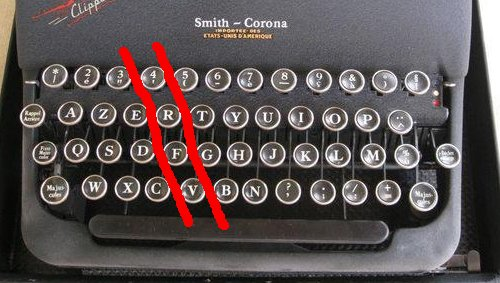
\includegraphics[height=5cm]{touches-diagonales.jpg}
\end{center}
\end{frame}

\begin{frame}{Solution : qwerty, azerty, …}
\begin{itemize}
  \item Placement des touches non optimisé
  \item Éviter le plus possible les coincements
  \item Quand même plus confortable qu'en abcd
\end{itemize}
\end{frame}

%%%%%%%%%%%%%%%%%%%%%%%%%%%%%%%%%%%%%%%%%%%%%%%%%%%%%%%%%%%%%%%%%%%%%%%%%%%%%%%
\section{Les claviers d'ordinateurs}
\begin{frame}
  \tableofcontents[sectionstyle=show/shaded, hideothersubsections]
\end{frame}

\subsection{Beaucoup d'électronique}
\begin{frame}{Beaucoup d'électronique}
\begin{itemize}
  \item Il n'y a presque plus de contrainte
  \item Le problème des barres qui se coincent n'existe plus :
  \begin{itemize}
    \item Les touches en diagonales sont inutiles
    \item Le qwerty, azerty, … sont obsolètes
  \end{itemize}
\end{itemize}
\end{frame}

\subsection{Touches en matrice}
\begin{frame}{Touches en matrice}
  Le TypeMatrix est un exemple de clavier ergonomique :
  \begin{center}
    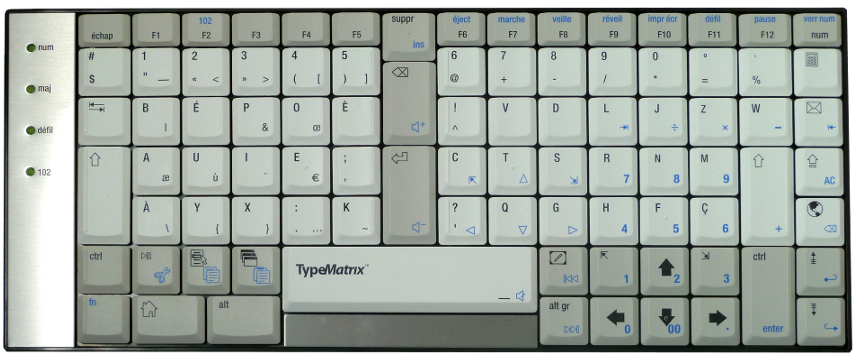
\includegraphics[height=4.5cm]{typematrix.png}
  \end{center}
\end{frame}

\subsection{Dispositions de type Dvorak}
\begin{frame}{Dispositions de type Dvorak}
  Principes établis par August \textsc{Dvorak} dans les années 1930 :
  \begin{itemize}
    \item Objectif : bouger le moins possible les doigts
    \item Symboles les plus courants sur la rangée du milieu
    \item Alterner souvent les mains
    \item Chaque main travaille équitablement
  \end{itemize}
  
  \bigskip
  \pause
  Pour réaliser une disposition de ce type :
  \begin{itemize}
    \item On calcule la fréquence de chaque symbole
    \item On se base sur des textes, du code source, etc.
  \end{itemize}
\end{frame}


%%%%%%%%%%%%%%%%%%%%%%%%%%%%%%%%%%%%%%%%%%%%%%%%%%%%%%%%%%%%%%%%%%%%%%%%%%%%%%%
\section{Dvorak bépo}
\begin{frame}
  \tableofcontents[sectionstyle=show/shaded, hideothersubsections]
\end{frame}

\subsection{Moins de mouvements de doigts}
\begin{frame}{Moins de mouvements de doigts}
\begin{center}
  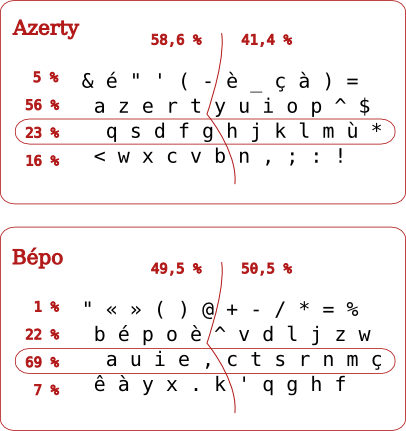
\includegraphics[height=6.5cm]{stats.png}
\end{center}
\end{frame}

\begin{frame}{Vidéo}
\url{http://www.dailymotion.com/video/x80kdk_azerty-vs-bepo_tech}
\end{frame}

\subsection{Plus de caractères disponibles}
\begin{frame}{Plus de caractères disponibles}
\begin{itemize}
  \item Les guillemets du français : << et >>
  \pause
  \item Les majuscules accentuées plus facile d'accès : É Ê È À Ç
  \pause
  \item Chiffres en exposant $ ^{123} $ ou indice $ _{456} $
  \pause
  \item Des symboles scientifiques : $ \neq \;  \leq \; \geq \; \pm \; \neg $ etc
  \pause
  \item Touches mortes :
  \begin{itemize}
    \item Exemple : \textasciicircum \hspace{1mm} + a $ \rightarrow $ â
    \item Accès à plein d'autres symboles
  \end{itemize}
\end{itemize}
\end{frame}

\subsection{Vitesse et endurance}
\begin{frame}{Vitesse et endurance}
\begin{itemize}
  \item La vitesse n'est pas le but premier
  \item Record de vitesse : en Dvorak US (200 mots par minute)
  \item Plus confortable donc moins de pauses
\end{itemize}
\end{frame}

\subsection{En pratique}
\begin{frame}{En pratique}
\begin{itemize}
  \item Taper à 10 doigts en aveugle (sans regarder le clavier)
  \item L'apprentissage peut être long mais c'est bénéfique
  \item Disponible de base sur GNU/Linux
  \item Archive nomade, pas besoin de droits d'administrateur
\end{itemize}
\end{frame}

%%%%%%%%%%%%%%%%%%%%%%%%%%%%%%%%%%%%%%%%%%%%%%%%%%%%%%%%%%%%%%%%%%%%%%%%%%%%%%%
\begin{frame}{Conclusion}
Les claviers actuels ne sont pas du tout confortables.

La disposition Dvorak bépo est adaptée pour la langue française.

Il existe des claviers ergonomiques comme le TypeMatrix.

\begin{center}
  \textbf{{\Large Des remarques, des questions ?}}
\end{center}
\end{frame}

\end{document}
